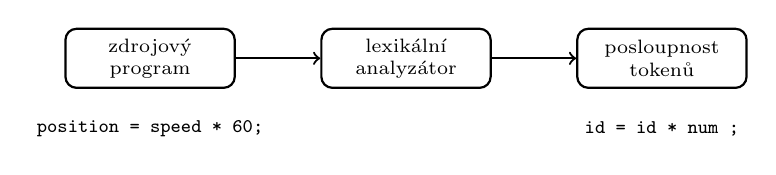
\begin{tikzpicture}[
    box/.style={
        draw,
        rounded corners,
        thick,
        align=center,
        font=\scriptsize,
        minimum width=2.15cm,
        minimum height=0.75cm
    },
    arrow/.style={->, thick}
]

    \node<3->[box] (src) at (0,0) {zdrojový\\program};
    \node<2->[box] (lex) at (3.25,0) {lexikální\\analyzátor};
    \node<4->[box] (tok) at (6.50,0) {posloupnost\\tokenů};

    \draw<3->[arrow] (src) -- (lex);
    \draw<4->[arrow] (lex) -- (tok);

    \node<6->[font=\scriptsize, align=center] at (0,-0.9)
        {\texttt{position = speed * 60;}};

    \node<6->[font=\scriptsize, align=center] at (6.50,-0.9)
        {\texttt{id = id * num ;}};

\end{tikzpicture}
